\chapter{Système proposé et protocole d'évaluation}
\label{chapitre:systeme}

Ce chapitre définit le système proposé et le protocole selon lequel il sera évalué en se
basant sur la période de référence individuelle, la branche HYPO, l'extension bidirectionnelle
exploratoire, la fusion des branches, les comparateurs et les métriques. Il relie aussi la
méthode au code exécuté~: le noyau HYPO, son évaluation, l'extension bidirectionnelle et
l'interface sont séparés afin qu'une modification de présentation ne change pas
silencieusement les résultats. Cette séparation répond aux dettes techniques que ces
travaux documentent dans les systèmes d'apprentissage automatique déployés
\citep{sculley2015hidden,amershi2019software,breck2017ml}. Les corpus et les campagnes
correspondantes sont décrits au Chapitre~\ref{chapitre:donnees}, alors que l'interface
proposée sera présentée au Chapitre~\ref{chapitre:interface}. La sortie étudiée est une \textbf{alerte comportementale} à
vérifier sur le terrain. Les termes de sensibilité et de faux positifs cliniques ne sont pas
employés pour l'évaluation synthétique, faute d'étalon vétérinaire.

% =====================================================================
\section{Vue d'ensemble du système}
% =====================================================================
La Figure~\ref{fig:architecture_modules} schématise l'architecture retenue du système
proposé. Les mesures brutes de chaque vache, stockées dans des fichiers CSV exportés du
système CowAlert, sont d'abord agrégées par intervalles de 15 minutes. Cette étape
calcule également la couverture de chaque intervalle, c'est-à-dire la proportion de la
période effectivement mesurée, qui sert ensuite à écarter les intervalles trop lacunaires.
Les mesures ainsi normalisées alimentent en parallèle les deux branches de détection, HYPO
pour les baisses persistantes et multivariées de l'activité, INSTABILITÉ pour les variations
désordonnées, dont les épisodes sont ensuite fusionnés en une notification de vérification ou
en une simple mise sous surveillance, qui signale la vache sans appeler de geste.

\begin{figure}[H]
  \centering
  \begin{tikzpicture}[
    box/.style={rectangle, draw=black!55, rounded corners=2pt, minimum height=1.20cm,
      text width=2.45cm, align=center, font=\normalsize, inner sep=4pt},
    branch/.style={box, minimum height=1.65cm},
    line/.style={line width=0.8pt, black!65},
    arrow/.style={line, -{Stealth[length=2.4mm, width=1.6mm]}}]
    \node[box, fill=profgray!10] (data) at (0,0) {CSV IceQube\\par vache};
    \node[box, fill=ifblue!10] (features) at (3.2,0) {Intervalles\\et couverture};
    \node[branch, fill=rulegreen!12] (hypo) at (6.4,1.05) {Branche HYPO\\12 h / 6 h};
    \node[branch, fill=loforange!12] (inst) at (6.4,-1.05) {Branche\\INSTABILITÉ\\3 h / 2 h};
    \node[box, fill=ifblue!8] (fusion) at (9.6,0) {Fusion\\hiérarchique};
    \node[box, fill=profgray!8] (action) at (12.8,1.05) {Notification de\\vérification};
    \node[box, fill=profgray!8] (surv) at (12.8,-1.05) {Surveillance\\d'instabilité};
    \coordinate (split) at (4.8,0);
    \coordinate (merge) at (8.0,0);
    \coordinate (dispatch) at (11.2,0);
    \draw[arrow] (data) -- (features);
    \draw[line] (features.east) -- (split);
    \fill[black!65] (split) circle (1.25pt);
    \draw[arrow] (split) -- (hypo.west);
    \draw[arrow] (split) -- (inst.west);
    \draw[line] (hypo.east) -- (merge);
    \draw[line] (inst.east) -- (merge);
    \fill[black!65] (merge) circle (1.25pt);
    \draw[arrow] (merge) -- (fusion.west);
    \draw[line] (fusion.east) -- (dispatch);
    \fill[black!65] (dispatch) circle (1.25pt);
    \draw[arrow] (dispatch) -- (action.west);
    \draw[arrow] (dispatch) -- (surv.west);
  \end{tikzpicture}
  \caption{Architecture du système, des mesures normalisées aux deux sorties de la fusion.}
  \label{fig:architecture_modules}
\end{figure}

Cette architecture est réalisée par une fonction unique du noyau logiciel,
\texttt{run\_pipeline\_one\_cow}, qui reçoit la série d'une seule vache et en retourne les
sorties de détection. Elle constitue le point d'entrée de toute la chaîne~: les campagnes
d'évaluation comme l'interface l'appellent, ce qui garantit qu'aucune ne peut appliquer une
règle qui lui serait propre. Ses opérations reprennent, dans l'ordre, les boîtes de la
Figure~\ref{fig:architecture_modules}~:
\begin{enumerate}
  \item normaliser les mesures et construire les intervalles, ce qui correspond au passage
  de la boîte \emph{CSV IceQube par vache} à la boîte \emph{Intervalles et couverture};
  \item matérialiser la séparation entre la période de référence et la période future, qui
  n'apparaît pas sur la figure mais conditionne tout ce qui suit;
  \item exécuter le comparateur Isolation Forest, employé comme point de comparaison et non
  représenté sur la figure, qui ne montre que la chaîne principale;
  \item calculer la branche HYPO, soit la boîte supérieure issue de l'embranchement;
  \item calculer la branche INSTABILITÉ, soit la boîte inférieure;
  \item appliquer la fusion choisie et espacer les notifications, soit la boîte
  \emph{Fusion hiérarchique};
  \item retourner les scores, épisodes, départs, notifications, types et priorités, que la
  figure résume par ses deux sorties, la notification de vérification et la surveillance
  d'instabilité.
\end{enumerate}
La chaîne appliquée au troupeau répète ce traitement sans partager de périodes de référence
entre les vaches.

% =====================================================================
\section{Période de référence individuelle}
% =====================================================================
La série d'intervalles de chaque vache est triée chronologiquement. Un intervalle est
admissible lorsque sa couverture atteint 25\,\% de sa durée~; la série ne débute toutefois
qu'au premier intervalle précédé de trois relevés valides consécutifs, le temps que le capteur
se stabilise. Les 60\,\% des intervalles admissibles
constituent la \textbf{période de référence}; les 40\,\% suivants forment la
\textbf{période future}. Les médianes de
référence sont calculées pour le même créneau horaire, avec repli sur la médiane globale de
la vache. Une deuxième référence considérée est la valeur observée au même créneau horaire le
jour précédent. Pour les familles
d'activité et le temps debout, le ratio le plus faible entre ces deux références est retenu;
pour le temps couché, le ratio le plus élevé est conservé. Ce choix sélectionne la référence
qui fait apparaître la variation la plus marquée, afin qu'une dégradation par rapport
à l'une des deux références ne soit pas masquée par l'autre. Les sorties sont forcées
à zéro pendant la période de référence et un intervalle dont la couverture est inférieure à 25\,\% ne
peut devenir candidat. Ce seuil figure parmi les paramètres soumis à l'analyse de
sensibilité de la Section~\ref{sec:sensibilite}. Ce découpage empêche une fuite directe de la période future vers la
référence. Il repose toutefois sur une hypothèse~: les premiers 60\,\% décrivent
suffisamment le fonctionnement habituel de la vache. Il ne garantit donc pas à lui seul
l'absence d'un épisode atypique, d'une dérive capteur ou d'un changement de conduite pendant
cette période.

% =====================================================================
\section{Branche HYPO~: baisse d'activité persistante}
\label{sec:hypo}
% =====================================================================
La branche HYPO cible la signature comportementale la mieux documentée de la boiterie, qui se
manifeste sous forme d'une réduction de l'activité locomotrice comme les pas, le mouvement et
les transitions, accompagnée d'une
augmentation du temps couché \citep{ito2010lying,blackie2011lying,chapinal2010measurement}.
Le détecteur recherche donc cette direction de changement plutôt qu'un écart quelconque.

Les pas, le \textit{Motion Index}, les transitions et les temps posturaux sont cumulés sur
12 heures. Pour les trois familles d'activité, le déficit est défini par
\begin{equation}
  \label{eq:deficit}
d_j(t)=\max(0,1-r_j(t)),
\end{equation}
où \(r_j(t)\) représente le ratio à la référence individuelle. Le changement postural
combine l'excès de temps couché et le déficit de temps debout. Le score est alors donné par la
relation suivante~:
\begin{equation}
  \label{eq:score_hypo}
S_H(t)=0{,}30d_{pas}+0{,}30d_{MI}+0{,}20d_{transitions}+0{,}20d_{posture}.
\end{equation}
Les trois premiers termes sont les instances de \(d_j(t)\) pour chacune des familles
d'activité~: \(d_{pas}\) pour les pas, \(d_{MI}\) pour le \textit{Motion Index} et
\(d_{transitions}\) pour les transitions posturales. Le quatrième, \(d_{posture}\), est le
terme combiné décrit ci-dessus, qui réunit l'excès de temps couché et le déficit de temps
debout. Les quatre varient entre zéro et un, zéro signifiant l'absence d'écart défavorable à
la référence.
Un candidat exige \(S_H\geq0{,}12\), pour au moins trois familles concordantes, l'implication des
pas ou du \textit{Motion Index}, une couverture suffisante et une position dans la période future.
Une famille est concordante lorsque son déficit atteint 10\,\%, seuil ramené à 5\,\% pour la
posture.
Une baisse progressive mesurée sur six heures renforce l'évidence. Le CUSUM représente la
somme cumulée unilatérale classique \citep{page1954continuous}. Il est défini par
\begin{equation}
  \label{eq:cusum}
C_t=\max(0,C_{t-1}+e_t-0{,}07),
\end{equation}
où \(e_t\) désigne l'évidence accumulée à l'intervalle
\(t\), nulle tant qu'aucun candidat n'est retenu, et \(C_{t-1}\) la valeur du cumul à
l'intervalle précédent. La soustraction d'une dérive constante de \(0{,}07\) fait redescendre
le cumul en l'absence d'évidence nouvelle, ce qui empêche une accumulation indéfinie. Le
cumul est unilatéral supérieur~: il part de zéro, ne peut jamais devenir négatif, et un
épisode se déclenche lorsqu'il franchit son seuil en montant.
Un épisode exige une persistance sur six heures et
\(C_t\geq1{,}20\). Deux notifications HYPO sont espacées d'au moins 24 heures. L'algorithme~\ref{alg:hypo}
résume cette logique de détection pour une vache.

\subsection{Formalisation et pseudocode}
\begin{algorithm}[H]
\caption{Détection HYPO d'une baisse d'activité persistante, pour une vache}
\label{alg:hypo}
\KwIn{Intervalles $X$ d'une vache, période de référence individuelle, paramètres $\theta$}
\KwOut{Épisodes, départs et notifications (alerte à vérifier, non diagnostique)}
\BlankLine
\PourChaque{famille de signaux $j$ parmi les pas, le \textit{Motion Index}, les transitions
et la posture}{
  Calculer la médiane de la période de référence par créneau horaire\;
  Se replier sur la médiane globale de la vache si le créneau est trop peu documenté\;
}
\BlankLine
\PourChaque{intervalle $t$ de la période surveillée}{
  Cumuler les totaux glissants sur $12$~h\;
  Calculer les ratios $r_j(t)$ aux références du créneau et de la veille, puis conserver
  celui qui correspond à la variation la plus marquée\;
  $d_j(t) \leftarrow \max\bigl(0,\ 1-r_j(t)\bigr)$
  \tcp*[l]{posture : excès couché, déficit debout}
  $S_H(t) \leftarrow 0{,}30\,d_{\text{pas}} + 0{,}30\,d_{\text{MI}}
   + 0{,}20\,d_{\text{transitions}} + 0{,}20\,d_{\text{posture}}$\;
  \Si{$S_H(t) \geq 0{,}12$, au moins trois familles concordantes, pas ou \textit{Motion Index}
  impliqués, et couverture suffisante}{
    $e_t \leftarrow S_H(t) + 0{,}35 \times (\text{baisse sur } 6\,\text{h})$
    \tcp*[l]{l'intervalle devient candidat}
  }
  \Sinon{
    $e_t \leftarrow 0$\;
  }
  $C_t \leftarrow \max\bigl(0,\ C_{t-1} + e_t - 0{,}07\bigr)$\;
  \Si{persistance du candidat sur $6$~h \KwEt $C_t \geq 1{,}20$}{
    Déclarer un épisode et enregistrer son départ\;
    Notifier au début de l'épisode, avec un délai réfractaire de $24$~h\;
  }
}
\end{algorithm}

\subsection{Implémentation de la persistance}
La persistance s'applique à l'intérieur de chaque branche, avant toute fusion, et non sur le
résultat d'une fusion brute. Chaque branche construit donc d'abord
ses propres candidats, son propre CUSUM et son propre épisode. Cette décision évite qu'une
instabilité courte doive durer six heures pour être reconnue ou qu'une baisse lente soit
déclenchée par deux heures de fluctuation. La fusion reçoit donc deux séries d'épisodes déjà
stabilisées.

Dans la branche HYPO, une fenêtre glissante de six heures doit contenir au moins 45\,\% des
candidats et le CUSUM doit franchir 1,20 par valeur croissante. Dans la branche INSTABILITÉ, la proportion minimale
est de 50\,\% sur deux heures et le CUSUM doit franchir 0,70. Ces règles sont déterministes et
testées séparément.

% =====================================================================
\section{Branche INSTABILITÉ~: mouvement disproportionné et posture fragmentée}
\label{sec:instabilite}
% =====================================================================
La branche INSTABILITÉ recherche une disproportion entre familles de signaux, et non une
hausse globale d'activité. Elle permet de calculer quatre
familles sur une fenêtre de trois heures: mouvement relatif aux pas, transitions relatives
aux pas, transitions relatives au temps postural et volatilité de la fraction couchée. Les
hausses des quatre familles sont pondérées respectivement par 0,35~; 0,30~; 0,20 et 0,15.

Un candidat doit satisfaire trois conditions~: son score atteint au moins 0,18; deux familles
au minimum réagissent, dont obligatoirement le mouvement relatif, corroboré par les
transitions, la fragmentation ou la posture; chaque famille retenue présente un changement
d'au moins 20\,\%.

Un filtre écarte ensuite l'activité générale~: une hausse conjointe des pas et du
\textit{Motion Index} d'au moins 15\,\%, avec un écart entre les deux inférieur à 20\,\% et
sans fragmentation, n'est pas retenue comme instabilité.

Le CUSUM emploie une dérive de 0,06 et un seuil de 0,70. La persistance exigée est de deux
heures et le délai réfractaire de 12 heures.

Les paramètres de la branche INSTABILITÉ sont des choix techniques exploratoires. Ils ont
été définis avant la campagne complète, puis soumis à une analyse de sensibilité. Ils ne sont
pas présentés comme des seuils physiologiques ou cliniquement optimaux.

% =====================================================================
\section{Fusion hiérarchique}
% =====================================================================
\subsection{Stratégies comparées}
Cinq stratégies de fusion sont comparées sur les mêmes événements:
\begin{enumerate}
  \item \textbf{HYPO}: seule la branche HYPO produit la sortie;
  \item \textbf{INSTABILITÉ}: seule l'instabilité produit la sortie;
  \item \textbf{OU}: toute branche active peut notifier;
  \item \textbf{HIÉRARCHIQUE}: l'hypoactivité, la convergence ou une séquence produit une
  alerte de vérification; l'instabilité isolée reste en surveillance;
  \item \textbf{SÉQUENTIELLE}: une alerte exige une instabilité suivie d'une hypoactivité
  entre 24 et 72 heures plus tard.
\end{enumerate}
La fusion hiérarchique est la configuration de référence de l'extension exploratoire. Sa
période réfractaire est de 12 heures. Une priorité 1 correspond à une surveillance
d'instabilité, une priorité 2 à une hypoactivité et une priorité 3 à une convergence ou une
séquence. La fusion hiérarchique n'est pas présupposée supérieure à HYPO: cette comparaison
fait partie des résultats. Le Tableau~\ref{tab:config_finale} présente les paramètres de
référence des deux branches.

\begin{table}[H]
  \centering
  \caption{Paramètres de référence des deux branches.}
  \label{tab:config_finale}
  \small
  \begin{tabular}{lcc}
    \toprule
    Paramètre & HYPO & INSTABILITÉ \\
    \midrule
    Agrégation & 12 h & 3 h \\
    Persistance & 6 h & 2 h \\
    Délai réfractaire & 24 h & 12 h \\
    Seuil de score & 0,12 & 0,18 \\
    Dérive CUSUM & 0,07 & 0,06 \\
    Seuil CUSUM & 1,20 & 0,70 \\
    Familles minimales & 3 & 2 \\
    Couverture minimale & 25\,\% & 25\,\% \\
    \bottomrule
  \end{tabular}
\end{table}

Ces valeurs sont des choix d'ingénierie~: l'agrégation de 12 heures suit le rythme journalier,
la persistance de 6 heures écarte les variations passagères, le délai réfractaire de 24 heures
limite les notifications à une par vache et par jour, trois familles sur quatre imposent une
concordance majoritaire et la couverture de 25\,\% est un plancher de qualité. Elles ont été
fixées avant la campagne d'évaluation, sans ajustement sur ses résultats, et la
Section~\ref{sec:sensibilite} en documente la robustesse locale. Elles n'ont pas pour autant
été choisies sur un jeu de développement indépendant du corpus évalué.

La sélection descriptive des fusions impose trois conditions de portée:
\begin{itemize}
  \item détection des scénarios de vérification d'au moins 60\,\%;
  \item surveillance de l'instabilité d'au moins 50\,\%;
  \item au moins 20\,\% d'événements atteignant le seuil IoU20.
\end{itemize}
Une fonction d'utilité secondaire récompense la détection et
pénalise fortement les contrôles, les confondants et la charge de fond. Ses poids sont des
choix d'ingénierie; elle ne représente pas une utilité clinique validée.

\subsection{Règle hiérarchique retenue}
La fusion hiérarchique est volontairement asymétrique. Une instabilité seule indique une
situation à surveiller, mais ne déclenche pas automatiquement une vérification prioritaire.
Une hypoactivité produit une notification de vérification. La priorité augmente lorsque les deux
branches convergent ou lorsqu'un départ HYPO est précédé d'un départ INSTABILITÉ dans la
fenêtre de 72 heures. Cette architecture empêche un simple pic de \textit{Motion Index} de
devenir une notification de vérification.

L'algorithme~\ref{alg:fusion} formalise la logique de fusion proposée pour une vache donnée.

\begin{algorithm}[H]
\caption{Fusion hiérarchique des branches HYPO et INSTABILITÉ, pour une vache}
\label{alg:fusion}
\KwIn{Intervalles $X$ d'une vache, période de référence individuelle, paramètres $\theta$}
\KwOut{Type d'alerte, priorité et notifications (alerte à vérifier, non diagnostique)}
\BlankLine
$\mathrm{hypo} \leftarrow \textsc{DétecterHypo}\bigl(X,\ \text{référence},\ \text{persistance}=6\,\text{h}\bigr)$
\tcp*[l]{baisse d'activité persistante}
$\mathrm{instab} \leftarrow \textsc{DétecterInstabilité}\bigl(X,\ \text{référence},\ \text{persistance}=2\,\text{h}\bigr)$
\tcp*[l]{mouvement disproportionné aux pas}
\BlankLine
\Si{$\mathrm{hypo}$ \KwEt $\mathrm{instab}$ récente ($\leq 72\,\text{h}$)}{
  priorité $\leftarrow 3$,\ \ type $\leftarrow$ \texttt{SEQUENCE}\;
}
\SinonSi{$\mathrm{hypo}$ \KwEt $\mathrm{instab}$}{
  priorité $\leftarrow 3$,\ \ type $\leftarrow$ \texttt{MIXTE}\;
}
\SinonSi{$\mathrm{hypo}$}{
  priorité $\leftarrow 2$,\ \ type $\leftarrow$ \texttt{HYPO}\;
}
\SinonSi{$\mathrm{instab}$}{
  priorité $\leftarrow 1$,\ \ type $\leftarrow$ \texttt{SURVEILLANCE}
  \tcp*[l]{à surveiller, sans vérification prioritaire}
}
\BlankLine
\Si{priorité $\geq 2$}{
  Émettre une notification\;
  Respecter un délai réfractaire de fusion de $12\,\text{h}$ entre notifications\;
}
\end{algorithm}

% =====================================================================

\section{Comparateurs Isolation Forest et Local Outlier Factor}
\label{sec:comparateurs}
% =====================================================================
Deux détecteurs d'anomalies non supervisés sont conservés comme points de comparaison. Ils
situent le détecteur temporel par rapport à des familles d'algorithmes répandues et
fournissent des points de comparaison reproductibles, sans produire de notifications
principales.

\subsection{Isolation Forest (IF)}
IF isole les observations rares en construisant des arbres de partition
aléatoire~: un point anormal, plus facile à séparer du reste, présente une profondeur
moyenne d'isolation plus faible \citep{liu2008isolation}. Les variables dérivées sont
d'abord mises à l'échelle par un \texttt{RobustScaler} de scikit-learn
\citep{sklearn_api}, sur l'intervalle inter-quantile 10--90, soit l'écart entre les
10\textsuperscript{e} et 90\textsuperscript{e} centiles, qui résiste aux distributions fortement asymétriques des signaux d'activité. Le
modèle est ajusté sur la période de référence de chaque vache, puis appliqué à l'ensemble de sa
série, de sorte qu'il décrive l'écart d'un intervalle par rapport au comportement
individuel appris. Les hyperparamètres figés sont rassemblés au
Tableau~\ref{tab:if_hyperparams}.

\begin{table}[H]
  \centering
  \caption{Hyperparamètres figés d'Isolation Forest (comparateur).}
  \label{tab:if_hyperparams}
  \small
  \begin{tabular}{p{0.30\textwidth}p{0.22\textwidth}p{0.36\textwidth}}
    \toprule
    Hyperparamètre & Valeur & Rôle \\
    \midrule
    Nombre d'arbres & 800 & Stabilité du score d'isolation \\
    Variables par arbre & 0,80 & Décorrélation des arbres \\
    Échantillonnage & \textit{bootstrap} & Diversité des sous-ensembles \\
    Contamination & 0,06 & Fraction supposée d'anomalies \\
    Graine aléatoire & 42 & Reproductibilité exacte \\
    Mise à l'échelle & RobustScaler 10--90 & Robustesse à l'asymétrie \\
    Ajustement & période de référence & Référence propre à chaque vache \\
    \bottomrule
  \end{tabular}
\end{table}

Les sorties \texttt{if\_score} et \texttt{if\_anomaly\_point}, ainsi que des colonnes de
compatibilité \texttt{pred\_lameness\_*}, restent disponibles. Elles alimentent l'ablation
du Chapitre~\ref{chapitre:resultats} et l'affichage, sans jamais définir la conclusion. Par
construction, IF repère un écart \emph{ponctuel} dans n'importe quelle
direction~; il ne modélise pas la référence horaire individuelle, la \emph{direction} ou
la \emph{persistance} d'une dégradation, qui sont précisément les propriétés recherchées par
la branche HYPO.

\subsection{Local Outlier Factor (LOF)}
LOF compare la densité locale d'un point à celle de ses voisins~: une
densité nettement plus faible que le voisinage signale une anomalie locale
\citep{breunig2000lof}. Il est exécuté en mode nouveauté dans le module d'ablation,
avec les mêmes indices d'entraînement et la même normalisation robuste que la comparaison
IF, afin que l'écart mesuré reflète l'algorithme et non un changement de
protocole. Sa complexité quadratique dans le cas général le rend moins apte au passage à
l'échelle, mais il peut capter des structures locales que les méthodes globales manquent.
Le Tableau~\ref{tab:if_vs_lof} compare les propriétés respectives d'IF et de LOF.

% =====================================================================
\section{Protocole d'évaluation}
% =====================================================================
Le module de campagne HYPO sélectionne les vaches admissibles, exécute une
référence propre et injecte les quatre profils de la campagne HYPO. Le module
d'ablation réutilise les mêmes fenêtres pour les cinq variantes comparées. Le
module d'extension bidirectionnelle étend ensuite le protocole aux douze scénarios
bidirectionnels. Le harnais garantit trois propriétés~: un placement reproductible des
perturbations, une attribution stricte de l'effet à l'injection, et le rejet de toute
campagne mal formée.

\subsection{Génération déterministe et exécution de référence}
La graine associée à chaque couple vache-scénario est dérivée au moyen de la fonction de
hachage cryptographique SHA-256, indépendamment de la variable d'environnement de hachage
de Python~; deux exécutions produisent donc exactement les mêmes injections. La position des profils est tournée entre les vaches pour ne pas
associer systématiquement une intensité à une période particulière. La fonction
d'injection renvoie une copie modifiée de la série et une table décrivant la fenêtre, les
changements cibles et la raison de conception, sans jamais altérer le fichier source.

Chaque vache est aussi exécutée \emph{sans} injection. Les nouveaux débuts de la série
injectée sont comparés aux débuts de cette référence avec une tolérance temporelle, et pour
la couverture comme pour l'IoU, le masque d'épisode de référence est soustrait intervalle
par intervalle du masque injecté. Cette étape est indispensable~: elle empêche de créditer
une injection lorsqu'une alerte identique aurait été produite par les données originales, et
c'est elle qui rend les métriques \emph{attribuables} (Section~\ref{sec:hypo}
du Chapitre~\ref{chapitre:systeme}).

\subsection{Attribution et contrôles bloquants}
La Figure~\ref{fig:hypo_cusum_example} sert de démonstration visuelle du mécanisme sur une
vache et une dégradation graduelle injectée après la période de référence. Le panneau~(a) montre que
le score comportemental $S_H(t)$ de l'exécution injectée s'élève au-dessus du seuil de
candidat et de l'exécution propre pendant la fenêtre injectée, puis redescend une fois
l'événement terminé. Le panneau~(b) montre que l'épisode détecté dans l'exécution
injectée se superpose à la fenêtre réelle. Un épisode plus court apparaît également dans
l'exécution sans injection, en raison d'une baisse naturellement présente dans les données.
L'évaluation ne retient donc que la portion supplémentaire produite par l'injection.

\begin{figure}[H]
  \centering
  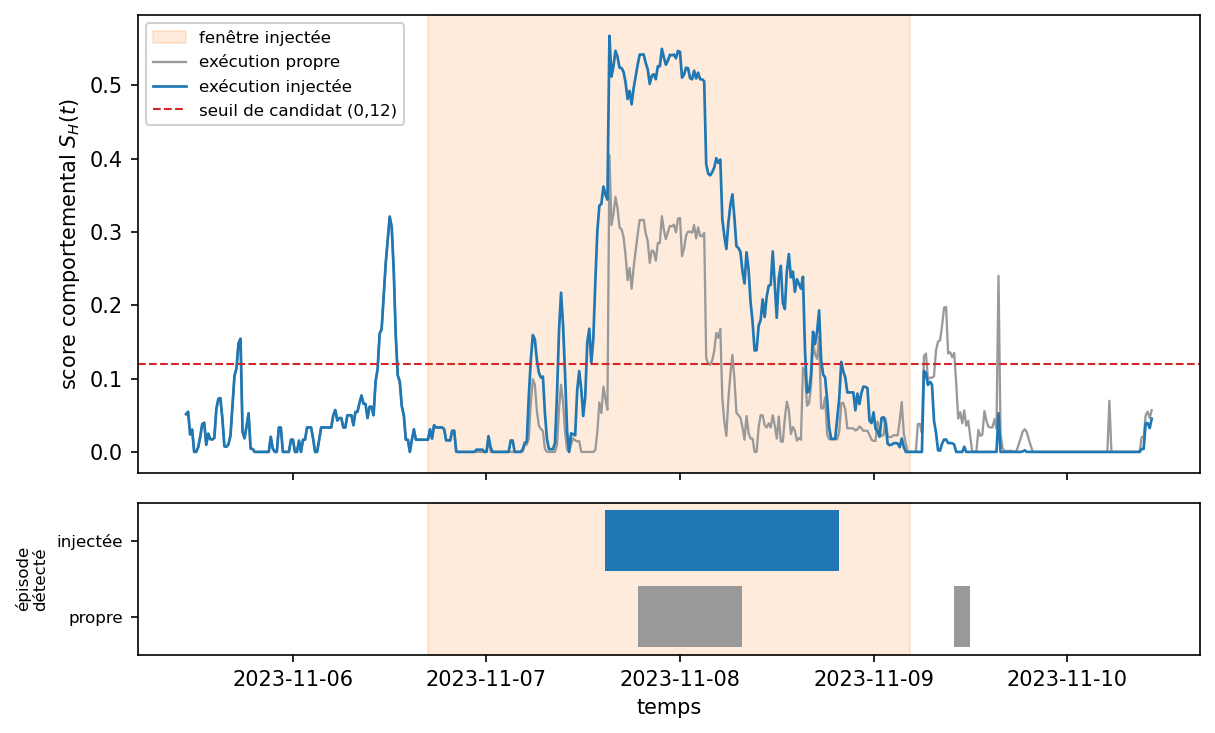
\includegraphics[width=0.95\textwidth]{figures/hypo_cusum_example.png}
  \caption{Détection attribuable au niveau de l'événement.}
  \label{fig:hypo_cusum_example}
\end{figure}

Avant tout calcul de résultat, le protocole vérifie l'unicité des identifiants d'événement,
leur non-chevauchement, leur placement strictement après la période de référence, la disponibilité des
signaux, la non-négativité des mesures, la conservation du temps postural total et l'absence
d'écriture dans le fichier source. Une campagne qui échoue à l'un de ces contrôles
n'alimente pas le manuscrit. La comparaison des fusions réutilise exactement les mêmes
vaches et les mêmes scénarios, de sorte que les écarts entre variantes ne tiennent qu'à la
règle de fusion.

% =====================================================================
\section{Métriques et analyses de sensibilité}
% =====================================================================
\subsection{Recouvrement temporel (IoU)}
La localisation d'un épisode est mesurée par l'intersection sur l'union
(\textit{Intersection over Union}, IoU), une métrique issue de la détection d'objets en
vision par ordinateur \citep{everingham2010pascal}, entre la fenêtre injectée et l'épisode
prédit~:
\begin{equation}
  \label{eq:iou}
\mathrm{IoU} = \frac{|\,\text{injecté} \cap \text{prédit}\,|}{|\,\text{injecté} \cup \text{prédit}\,|},
\end{equation}
exprimée en nombre d'intervalles de 15 minutes. Une valeur de~1 indique une superposition
parfaite, alors qu'une valeur de~0 indique une absence de chevauchement. Le seuil IoU~$\geq0{,}20$ retient
les épisodes raisonnablement localisés~; il est nettement plus strict que le simple
recouvrement, qui ne compte qu'un chevauchement non nul.

Le recours à l'IoU plutôt qu'au seul recouvrement tient à ce qu'il sanctionne les deux écarts
possibles. Un chevauchement non nul est acquis dès qu'un intervalle est partagé, quelle que
soit la durée de l'épisode prédit~: une alerte qui couvrirait toute la période surveillée
obtiendrait le même crédit qu'une alerte parfaitement ajustée. En rapportant l'intersection à
l'union, l'IoU pénalise aussi bien l'épisode trop court que l'épisode trop long. Il mesure donc
la localisation, là où le recouvrement ne mesure que la présence.

Le seuil retenu est délibérément plus bas que celui de~0,5 usuel en détection d'objets, et
deux raisons le justifient. D'une part, la fenêtre injectée possède des bornes nettes par
construction, alors qu'une dégradation comportementale réelle n'en a pas~: exiger un
recouvrement élevé reviendrait à demander au détecteur de retrouver des limites qui n'existent
que dans le protocole. D'autre part, la chaîne de détection agrège les signaux sur plusieurs
heures et impose une persistance avant de déclarer un épisode~; sa réponse est nécessairement
étalée par rapport à la fenêtre, et un seuil sévère pénaliserait le lissage qui fait sa
robustesse.

Cette métrique n'est jamais lue seule. Un IoU faible peut correspondre à une alerte qui
commence au bon moment mais se prolonge au-delà de l'événement, ce qui reste exploitable en
ferme, comme à une alerte franchement décalée, qui ne l'est pas. Les résultats la présentent
donc systématiquement à côté de la couverture attribuable et du nouveau départ~: la première
indique si le système a réagi, le second s'il a réagi par un épisode distinct de son
comportement habituel, et l'IoU indique où il a réagi.

\subsection{Métriques attribuables et unité statistique}
Une détection est attribuable seulement si l'exécution injectée ajoute un intervalle ou un
départ absent de l'exécution propre. Pour HYPO, les résultats distinguent un nouveau départ,
une couverture attribuable, un IoU~$\geq0{,}20$, le meilleur IoU, un délai et une notification
de fond. Ces entités sont volontairement reliées à des notions connues: la couverture joue le
rôle d'un rappel événementiel permissif, le nouveau départ joue le rôle d'un rappel
événementiel strict, l'IoU mesure la localisation temporelle et les notifications de fond
mesurent la charge opérationnelle. Pour
l'extension, les métriques ajoutent les taux de surveillance, de contrôle et de confusion. Les
synthèses inférentielles utilisent la vache comme unité; les lignes de 15 minutes ne sont
jamais des sujets indépendants.

Comparer les départs des deux exécutions suppose de décider quand deux départs proches sont le
même événement. Cette comparaison admet une tolérance temporelle d'une heure~: un départ de
l'exécution injectée situé à moins d'une heure d'un départ de l'exécution propre est considéré
comme le même déclenchement et n'est pas crédité. Ce choix est conservateur, et son effet est
mesuré plutôt que supposé. Sans tolérance, deux départs distants d'un seul intervalle
compteraient comme distincts et le taux de nouveau départ atteindrait 50,0\,\% au lieu de
43,2\,\%~; avec deux heures, il descendrait à 38,6\,\%. Ce balayage de la tolérance est
reproductible par un script nommé
\path{scripts/compute_match_tolerance_sensitivity.py}. La valeur retenue n'est donc pas celle
qui flatte le résultat. La couverture attribuable et l'IoU ne dépendent pas de cette décision,
puisqu'elles se calculent sur les intervalles attribuables sans jamais apparier de départs~:
elles restent inchangées sur toute la plage et servent de témoin à cette vérification.

La dépendance temporelle entre les intervalles successifs est quantifiée sur le corpus par le
temps d'autocorrélation intégré $\tau$ et par la taille d'échantillon effective
$n_{\text{eff}}=n/\tau$, où $n$ désigne le nombre d'observations disponibles et $\tau$ le temps
d'autocorrélation exprimé en nombre de pas d'échantillonnage. Les résultats descriptifs
correspondants seront présentés à la Section~\ref{subsec:statistiques_corpus}. Comme les fenêtres
glissantes voisines partagent une grande partie de leurs mesures, c'est la vache qui constitue
l'unité de rééchantillonnage. Le calcul est reproductible par un script nommé
\path{scripts/compute_correlation_time.py}.

La détection peut aussi être résumée, au niveau de l'événement, par un score F1. Les
dégradations graduelles constituent les positifs attendus, tandis que les contrôles brefs
constituent les négatifs attendus. Un vrai positif correspond à un événement graduel détecté de
façon attribuable, alors qu'un faux positif représente un contrôle bref alerté à tort. D'autre
part, un faux négatif correspond à un événement graduel manqué, tandis qu'un vrai négatif
correspond à un contrôle correctement rejeté. Le score F1 est la moyenne harmonique de la
précision et du rappel correspondants. Cela dit, cette synthèse reste complémentaire: elle
n'intègre ni la charge de fond ni la qualité fine de localisation.

\subsection{Analyses de sensibilité prévues}
L'analyse OFAT évalue
20 variantes des paramètres de HYPO, obtenues en ne modifiant qu'une valeur à la fois.
Une analyse plus restreinte modifie ensuite l'agrégation, la persistance et les seuils de la
branche INSTABILITÉ. Les deux analyses servent à détecter une dépendance excessive aux
valeurs de référence, non à optimiser les paramètres sur les événements évalués.

Deux analyses exploratoires complètent ce dispositif sans modifier la configuration
principale. La première estime, uniquement sur la période de référence de chaque vache, un facteur
proportionnel à l'écart-type de son score, puis ré-exécute la campagne avec un seuil
individualisé. La seconde fait varier le seuil de score HYPO de 0,04 à 0,20, une plage qui encadre
symétriquement la valeur retenue de 0,12, en conservant
les mêmes vaches, fenêtres, injections et autres paramètres. Elle décrit conjointement la
réponse aux événements graduels et la charge produite par les exécutions propres. Ces
analyses ont été ajoutées après la campagne principale~: elles servent à examiner des
hypothèses et non à sélectionner rétrospectivement une nouvelle valeur de seuil.

% =====================================================================
\section{Reproductibilité et organisation logicielle}
% =====================================================================
Les configurations et les sorties sont exportées en fichiers CSV. Les tests vérifient le placement
postérieur à la période de référence, la conservation posturale, la fusion et les contrats
de sortie. L'Annexe~\ref{annexe:validation} fournit les commandes de reproduction. Cette
démarche rejoint les recommandations sur la reproductibilité en apprentissage automatique et
la gestion FAIR des données \citep{pineau2021improving,wilkinson2016fair}.

\subsection{Organisation du logiciel}
Le Tableau~\ref{tab:modules} récapitule les composants logiciels et les campagnes de
reproduction qui produisent les sorties du mémoire.

\begin{table}[H]
  \centering
  \caption{Composants logiciels et campagnes de reproduction du mémoire.}
  \label{tab:modules}
  \begingroup
  \small
  \setlength{\tabcolsep}{5pt}
  \begin{tabular}{p{0.31\textwidth}p{0.62\textwidth}}
    \toprule
    Composant & Rôle \\
    \midrule
    Chargement des données & Lecture CSV, colonnes et horodatage. \\
    Dérivation des variables & Agrégation 15 min, couverture et variables dérivées. \\
    Branche HYPO & Référence individuelle, score, CUSUM et persistance. \\
    Branche INSTABILITÉ & Mouvement disproportionné, posture fragmentée et fusion. \\
    Pipeline troupeau & Orchestration par vache et agrégation troupeau. \\
    Comparateur Isolation Forest & Référence non supervisée pour l'ablation et l'interface. \\
    Évaluation HYPO & Campagne principale après la période de référence. \\
    Ablation HYPO & Comparaison avec IF, LOF et le comparateur pédométrique. \\
    Sensibilité HYPO & Analyse OFAT sans sélection de nouvelle configuration. \\
    Test de stress HYPO & Formes moins favorables à aire d'enveloppe appariée, sans nouveau réglage. \\
    Calibration par vache & Test exploratoire d'un seuil individualisé. \\
    Courbe détection-charge & Compromis entre détection attribuable et charge de fond. \\
    Évaluation bidirectionnelle & Scénarios HYPO, INSTABILITÉ, séquence et contrôles. \\
    Sensibilité de la fusion & Comparaison des règles de fusion et sensibilité technique. \\
    Analyse IceTag-SLS synchronisée & Confrontation exploratoire aux scores locomoteurs. \\
    Interface Streamlit & Visualisation individuelle, classement troupeau et export des alertes. \\
    Tests automatisés & Tests unitaires, invariants et non-régression. \\
    \bottomrule
  \end{tabular}
  \endgroup
\end{table}

Les fichiers exécutables exacts sont répartis par responsabilité: \texttt{core/} porte le
noyau de détection, soit les variables dérivées, les deux branches et leur
fusion, \texttt{validation\_hypo/} et \texttt{validation\_hybrid/} portent les
campagnes reproductibles, \texttt{scripts/} regroupe les tâches de soutien, \texttt{app.py}
et \texttt{ui/} portent l'interface, et \texttt{tests/} regroupe les contrôles automatisés.
Les scripts réutilisent les campagnes existantes sans introduire de logique d'alerte
parallèle.

\subsection{Technologies et dépendances}
Les principales dépendances sont figées dans le fichier \path{requirements.txt} et leurs
versions exactes sont reportées au Tableau~\ref{tab:technologies}, en annexe. Elles servent à
reconstruire l'environnement et à garantir la reproductibilité numérique~; elles ne constituent
pas un résultat scientifique.
Les comparateurs IF et LOF proviennent de \texttt{scikit-learn}
\citep{sklearn_api}, les tests statistiques de \texttt{SciPy} \citep{virtanen2020scipy},
et l'interface de \texttt{Streamlit}; la manipulation des données et le calcul numérique
reposent sur \texttt{pandas} \citep{mckinney2010data} et \texttt{NumPy} \citep{harris2020array}.


\subsection{Évaluation du temps d'exécution}
L'évaluation reconstruit les variables, exécute le comparateur Isolation Forest, les règles
IF comparatives, HYPO, INSTABILITÉ et la fusion hiérarchique. Chaque étape est chronométrée avec
une horloge monotone. Cinq répétitions sont effectuées sur l'ensemble du corpus principal et la concaténation
des sorties intervalle est incluse. Le résultat canonique est la médiane des cinq durées; les
valeurs minimale et maximale sont conservées pour rendre visible la variabilité de la machine.
Cette évaluation du temps d'exécution documente la faisabilité du prototype sur l'ordinateur
utilisé, non un temps garanti en production.

\subsection{Tests et traçabilité}
La suite automatisée contient 136 tests et couvre le chargement, les variables dérivées,
les deux détecteurs, les valeurs de référence du Tableau~\ref{tab:config_finale}, les cinq fusions
et l'asymétrie de la règle hiérarchique, les injections, les contrôles après la période de référence,
l'isolement de la période de référence vis-à-vis de la période future et le caractère unilatéral du cumul,
l'appariement de l'aire d'enveloppe, l'analyse de sensibilité, l'analyse SLS exacte et le démarrage de
Streamlit. Les résultats sont
écrits dans des fichiers tabulaires dont la provenance est explicite. Le succès des tests
atteste la cohérence logicielle et sécurise la reproduction des résultats.

Chaque résultat suit un cycle de vie traçable en trois étapes~: 1-~une commande de
reproduction exécute un module d'évaluation, qui écrit des fichiers CSV et JSON~; 2-~un
manifeste SHA-256 fige ces sorties ainsi que l'empreinte du corpus confidentiel~; 3-~un
script dédié les transforme automatiquement en figures de résultats du manuscrit. Aucun résultat empirique n'est accepté sans comparaison
à son artefact source. Une modification du code, des données ou des paramètres impose donc
une nouvelle exécution et un nouveau manifeste, de sorte que le PDF du mémoire ne constitue jamais
à lui seul la trace de référence de l'expérience. La Figure~\ref{fig:repro_chain} illustre cette chaîne de reproductibilité.

\begin{figure}[H]
  \centering
  \begin{tikzpicture}[
    procbox/.style={rectangle, draw=black!55, rounded corners=2pt, align=center,
      minimum height=1.55cm, text width=2.15cm, font=\normalsize, inner sep=4pt},
    arrow/.style={-{Stealth[length=2.4mm, width=1.6mm]}, line width=0.8pt, black!65}]
    \node[procbox, fill=profgray!10] (csv) at (0,0)
      {\textbf{1}\\Données IceQube};
    \node[procbox, fill=ifblue!10] (split) at (3.0,0)
      {\textbf{2}\\Séparation temporelle};
    \node[procbox, fill=loforange!10] (inject) at (6.0,0)
      {\textbf{3}\\Injection future};
    \node[procbox, fill=rulegreen!12] (detect) at (9.0,0)
      {\textbf{4}\\HYPO et fusion};
    \node[procbox, fill=ifblue!8] (attrib) at (12.0,0)
      {\textbf{5}\\Attribution des sorties};
    \node[procbox, fill=profgray!10] (out) at (12.0,-2.35)
      {\textbf{6}\\Résultats CSV};
    \node[procbox, fill=profgray!10] (fig) at (9.0,-2.35)
      {\textbf{7}\\Figures du mémoire};
    \node[procbox, fill=rawred!12] (sha) at (6.0,-2.35)
      {\textbf{8}\\Manifeste SHA-256};
    \draw[arrow] (csv) -- (split);
    \draw[arrow] (split) -- (inject);
    \draw[arrow] (inject) -- (detect);
    \draw[arrow] (detect) -- (attrib);
    \draw[arrow] (attrib) -- (out);
    \draw[arrow] (out) -- (fig);
    \draw[arrow] (fig) -- (sha);
  \end{tikzpicture}
  \caption{Chaîne de reproductibilité, des données brutes au manifeste SHA-256.}
  \label{fig:repro_chain}
\end{figure}

Le manifeste ferme la chaîne en rendant toute modification d'un artefact détectable. Il
atteste l'identité des fichiers reproduits et complète les contrôles méthodologiques décrits
dans le chapitre des résultats.
